% UPDATED BY MARCUS SCHAGERBERG, 2023
% CREATED BY WOLFGANG AHRENDT, 2021

% WRITTEN BY FELIX JÖNSSON, 2023
This section lays the theoretical foundation for the essential concepts that underpin the implementation of our agent-based traffic model in Unity. It covers a variety of topics, including specific mathematical functions, code design principles, pathfinding algorithms, and the theoretical aspects of software development project management frameworks. By establishing a solid understanding of these core concepts, readers will be better prepared to grasp the intricacies of the traffic simulation presented later in this thesis.

% WRITTEN BY FELIX JÖNSSON, 2023
\section{Unity}

A game engine is a software framework designed to facilitate the creation of video games by providing the most commonly needed functionalities. These include complex tasks such as physics calculations, animation, rendering, and artificial intelligence. The advantage of using a pre-existing game engine is that it allows developers to focus on the unique aspects of their game and accelerates the development pipeline, as they do not have to code these complex systems from scratch.

Unity is a game engine initially released for Mac OS X in 2005 at the Apple Worldwide Developers Conference\cite{macworld2005}. The CEO of the company has said that the mission was to democratize game development, making it widely accessible to a broad audience\cite{polygon2014}. By 2022, the company had secured a significant market share of 38\%, signifying its wide acceptance and popularity within the industry\cite{slashdata2022}.

Unity can be used to produce both 2D and 3D environments, and it offers native support for a wide variety of platforms and operating systems. Although there is a wealth of underlying theory supporting the engine, of which the most prominent is considered to be the Component-Based Object Model. Development in Unity is centered around so-called GameObjects, which serve as the base class for all entities in Unity scenes. These GameObjects can then receive different components, which can take the form of a wide range of things, such as scripts, textures, cameras, and so on. This pattern allows for a flexible and modular development approach, as many GameObjects can reuse the same component while customizing each component parameter to their specific requirements.

Another central underlying theory is that of Event-Driven Programming and the implementation of a so-called game loop\cite{gameprogrammingpatterns2023}. By using an event-centric communication method for many of its native systems such as input handling and collision detection, components such as scripts can define methods that hook onto the event architecture. These can then respond to specific events such as "OnCollisionEnter", which is called when a collision occurs\cite{unityManualExecutionOrder2023}\cite{unityManualEventFunctions2023}. This Event-Driven approach works in symbiosis with the theory of a game loop. A game loop is a ubiquitous architecture technique used within the game engine sphere. The basic concept is that an update event occurs each frame, also called a tick, where all GameObjects and their components have the opportunity to react and update themselves according to the current state of their environment. Since these updates occur with high frequency, often many times per second, this allows the game to simulate real-time behavior.



\newcommand{\timeconstraint}{, \quad 0 \le t \le 1}
\newcommand{\lerp}{\rightarrow}
\newcommand{\p}[1]{P\textsubscript{#1}}

% Marcus Schagerberg
\section{Bézier curves}
    A Bézier curve is a parametric curve between two points, that curves according to a set of intermediate points. The points are called control points, where the first and last point are the endpoints of the curve. A linear Bézier curve only has two points, which means that it is a line between the points. It is defined by the following function:

    $$
        P(t) = (1-t)^2P_0 + 2t(1-t)P_1 + t^2P_2 \timeconstraint
    $$

    The parameter $t$ is the ratio along the line, with $t = 0$ and $t = 1$ marking the endpoints. This is what is known as linear interpolation in mathematics. A linear Bézier curve is therefore simply a linear interpolation between the points $P_0$ and $P_1$. Let's define this as $P_0 \lerp P_1$. The quadratic Bézier curve consists of two linear interpolations:
    
    $$ A) \quad P_0 \lerp P_1$$
    $$ B) \quad P_1 \lerp P_2 $$
    
    It is then defined as the linear interpolation between these points, i.e $ A \lerp B $. All linear interpolations in this case depend on the same $t$, which is what creates the curvature of the Bézier curves.

    Since a quadratic Bézier curve has three points, it will have two endpoints as well as an additonal control point between them. By moving the control point, the shape of the Bézier curve can be altered. This is presented with the following examples, the first three of which have static endpoints demonstrating how the middle control point can be used to form the curve. The final example eludes to the fact that the control points can be placed anywhere without the requirement of any order.

    \begin{figure}[H]
        \begin{tabular}{cc}
            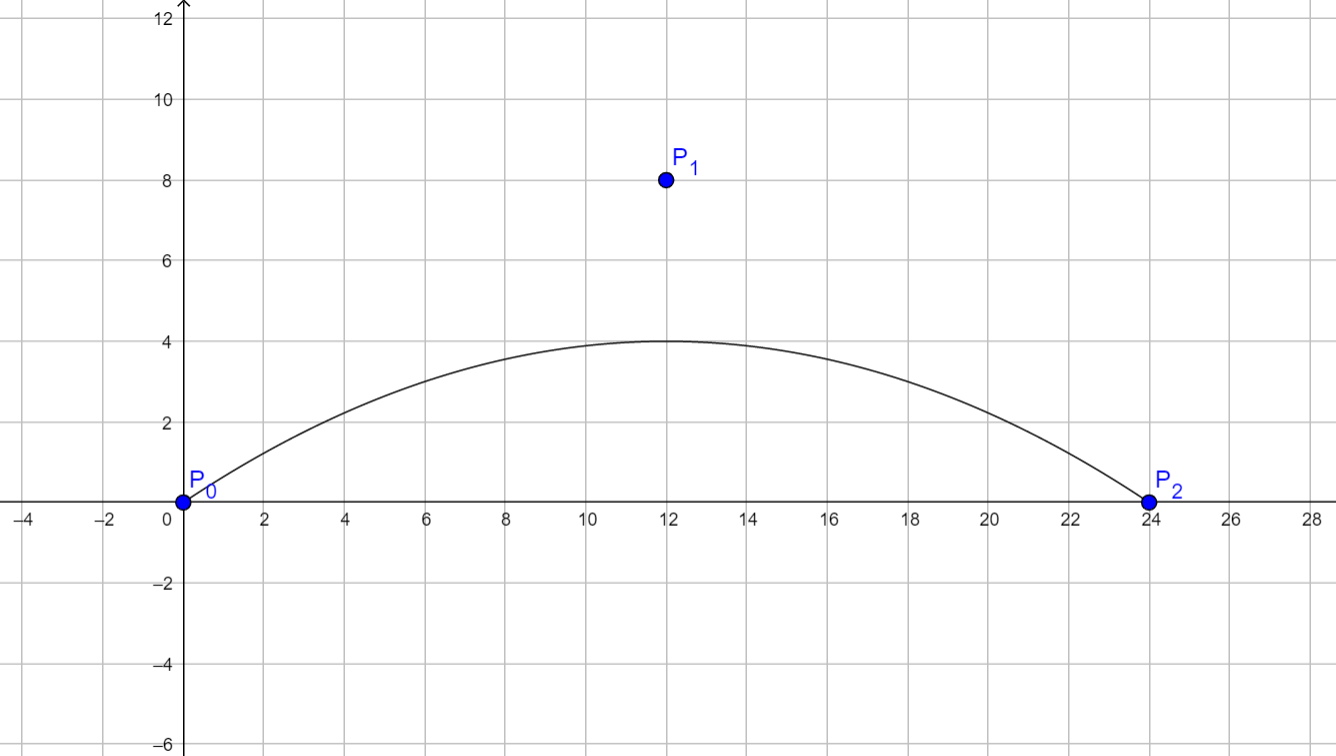
\includegraphics[width=0.5\linewidth]{figures/theory/bezier_curves/quadratic1.png} & 
            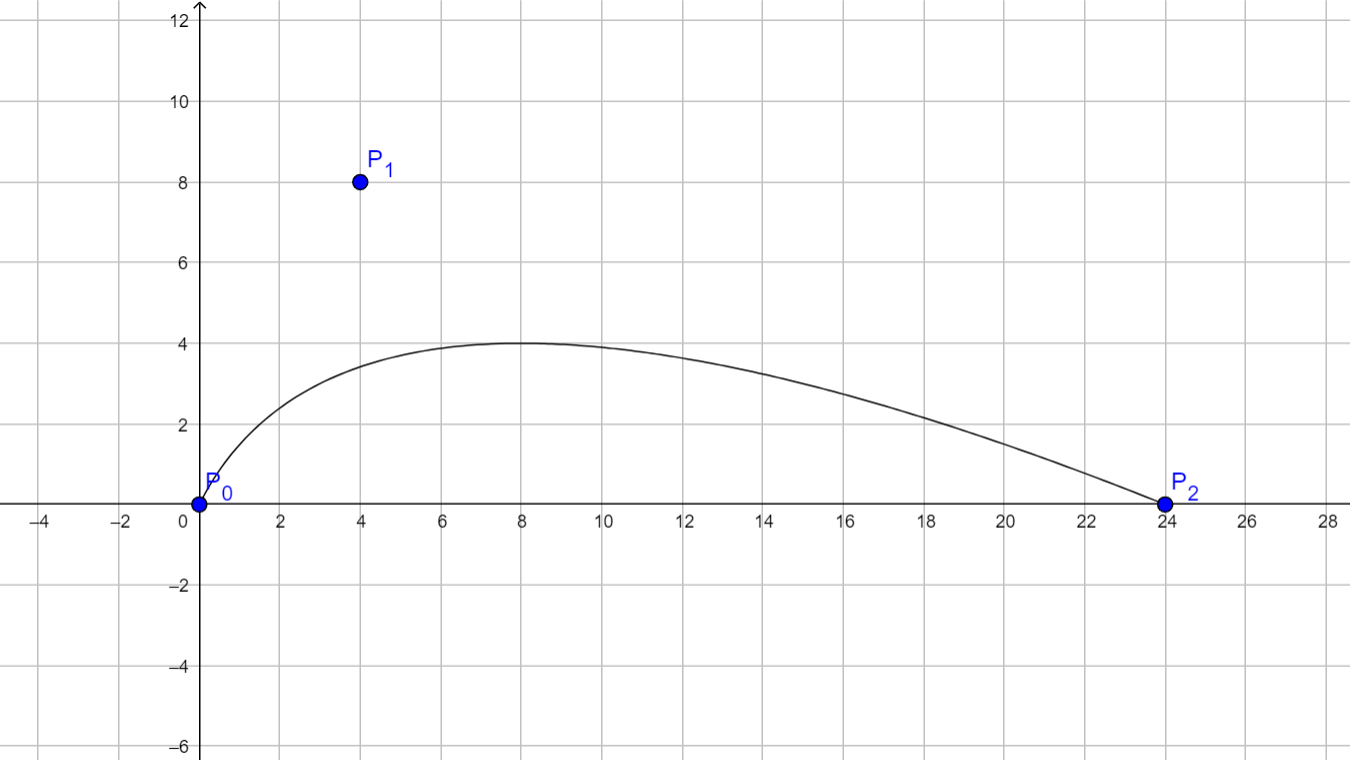
\includegraphics[width=0.5\linewidth]{figures/theory/bezier_curves/quadratic2.png} \\
            
            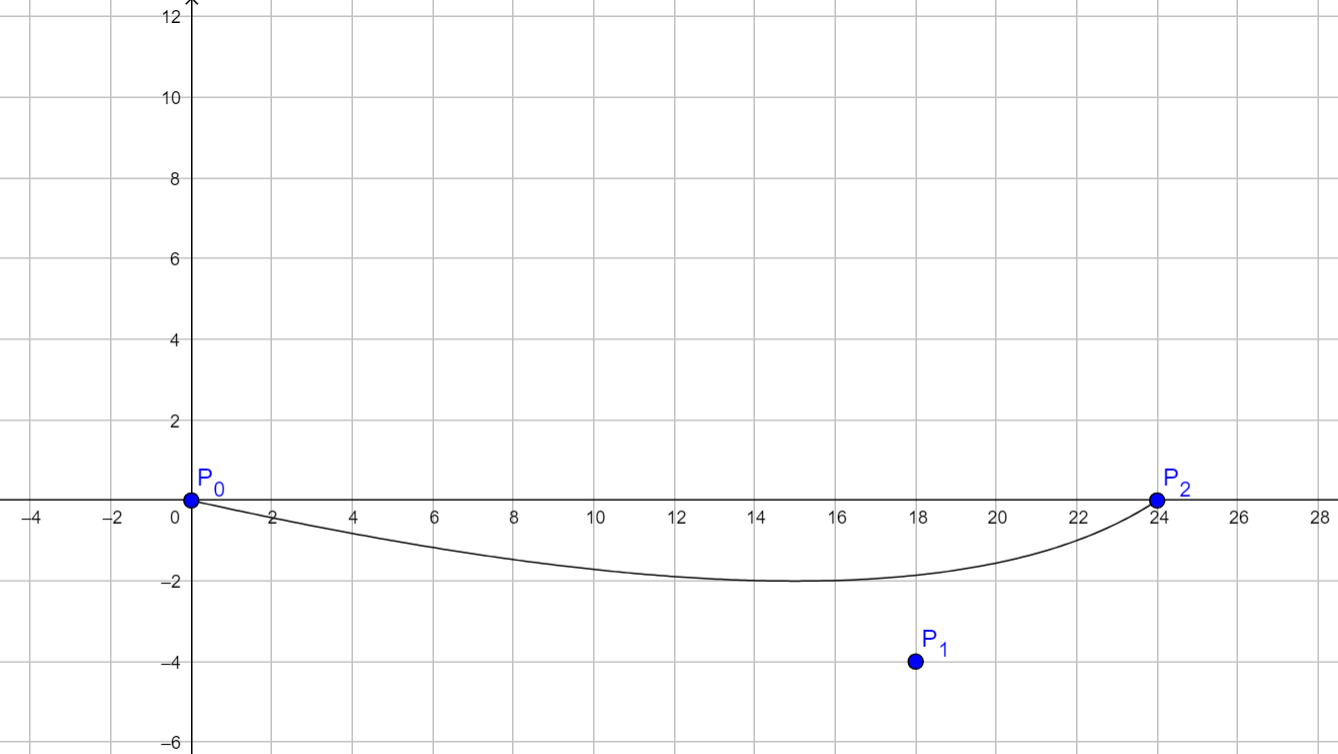
\includegraphics[width=0.5\linewidth]{figures/theory/bezier_curves/quadratic3.png} & 
            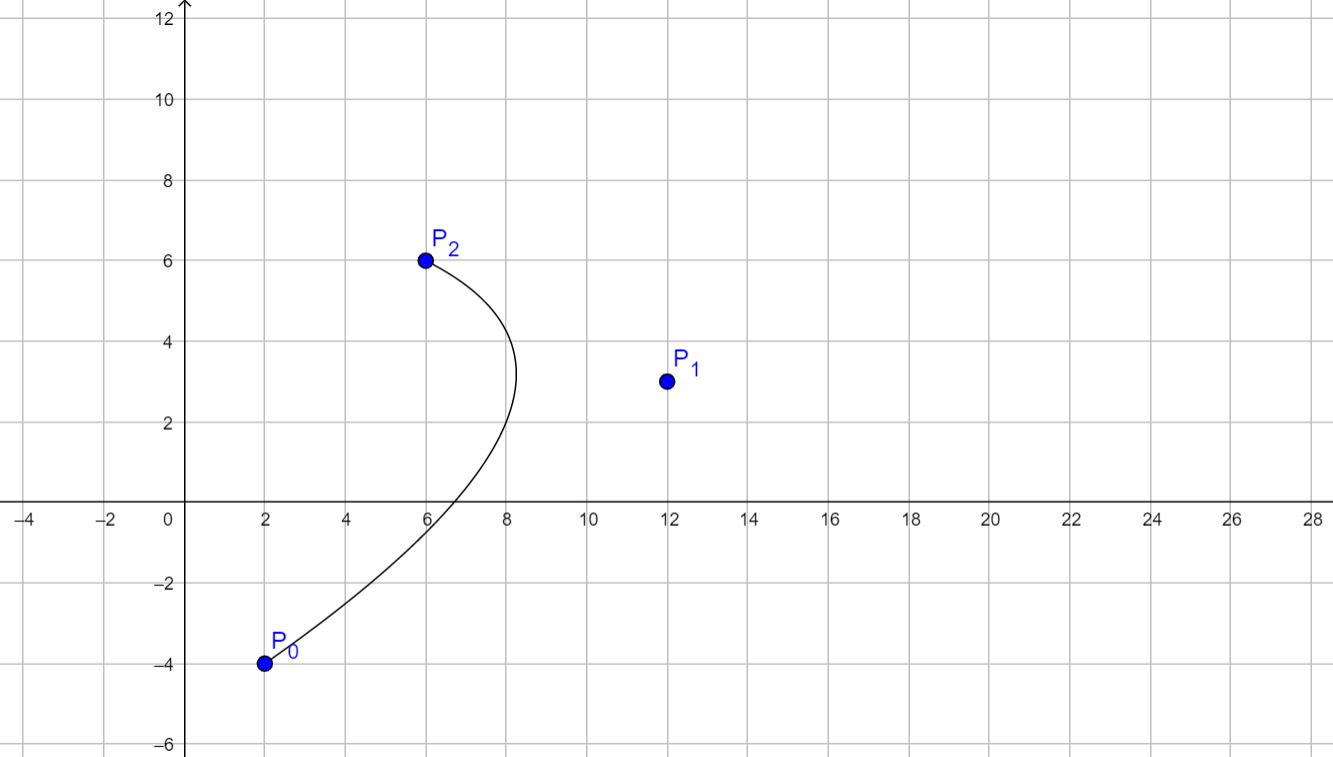
\includegraphics[width=0.5\linewidth]{figures/theory/bezier_curves/quadratic4.png}
        \end{tabular}
        \caption{Four examples of quadratic Bézier curves}
    \end{figure}

    
    
    % Hannes Kaulio and Marcus Schagerberg
    \subsection{Cubic Bézier Curve}
        A cubic Bézier curve expands on the quadratic curve in the same fashion as the quadratic expanded on the linear Bézier curve, adding another layer of linear interpolations. A cubic Bézier curve has four control points, two of which are endpoints.
        
        \inlineimage{figures/theory/bezier_curves/bezier_curve.png}{Cubic Bézier curve with control points \p{0}, \p{1}, \p{2} and \p{3}}{0.5}
    
        The cubic Bézier curve can be defined by the formula\cite{Cubic-Bézier-Curves}: 
        $$
            P(t) = (1-t)^3P_0 + 3t(1 - t)^2P_1 + 3t^2(1 - t)P_2 + t^3P_3 \timeconstraint
        $$
        Properties of the Cubic Bézier curve relevant to this paper are the following:
        \begin{enumerate}
            \item The endpoints \p{0} and \p{3} lay on the curve
            \item The curve is continuous, infinitely differentiable, and the second derivatives are continuous.
            \item The tangent line to the curve at the point \p{0} is the line \p{0}\p{1}. The tangent to the
        curve at the point \p{3} is the line \p{2}\p{3}.
            \item Both \p{1} and \p{2} lay on the curve only if the curve is linear.
            \item A Bézier curve is contained within the convex hull of the control points. For the application in Unity, this means that a Bézier curve is completely contained within the bounding box created by its control points.
        \end{enumerate}

    % Marcus Schagerberg
    \subsection{De Casteljau's algorithm}
        In 1959 the french mathematician Paul de Casteljau constructed an algorithm for dividing a Bézier curve into two. The union of these Bézier segments is equivalent to the original curve.
    
    % Marcus Schagerberg
    \subsection{Bézier Clipping}
        Finding the intersection points between two Bézier paths is not as straight forward as for something like two lines. To solve this, an algorithm called Bézier clipping explained in \cite{bezier-clipping} can be used. It utilises the convex hull property of Bézier curves - and therefore Bézier paths - as well as de Casteljau's algorithm for splitting curves. An implementation for finding all intersection points between two Bézier paths using Bézier clipping is outlined below.

        \vspace{1cm}
        \begin{algorithmic}
            \State $intersections \gets$ Empty list
            \State $epsilon \gets$ A value >0 small enough for the desired accuracy
            \Procedure{FindBezierPathIntersections}{$A, B$}
                \If{$A.BoundingBox$ does not intersect $B.BoundingBox$}
                    \State \Return
                \EndIf

                \If{$A.BoundingBox.Size$ + $B.BoundingBox.Size < epsilon$}
                    \State $intersections \gets$ Midpoint between A and B
                    \State \Return
                \EndIf

                \State $A_1, A_2 \gets SplitWithDeCasteljau(A, 0.5)$
                \State $B_1, B_2 \gets SplitWithDeCasteljau(B, 0.5)$

                \State $FindBezierPathIntersections(A_1, B_1)$
                \State $FindBezierPathIntersections(A_1, B_2)$
                \State $FindBezierPathIntersections(A_2, B_1)$
                \State $FindBezierPathIntersections(A_2, B_2)$
            \EndProcedure
        \end{algorithmic}
        \vspace{1cm}

        Worth noting is the $Midpoint$, which is one of many possible approximations of the intersection point. For a small enough $epsilon$, the approximation used is trivial as the segments approaches points as $epsilon$ approaches 0.

    % Hannes Kaulio and Marcus Schagerberg
    \subsection{Composite Bézier curve}
        A composite Bézier curve is a spline made out of Bézier curves. The series of Bézier curves are joined together end to end with the start point of one curve coinciding with the end point of the other curve. This is used in the projects as it allows for chaining of cubic Bézier path segments creating a spline. 

% WRITTEN BY HANNES KAULIO AND FELIX JÖNSSON, 2023
% Hannes Kaulio + Felix 
\section{A* Algorithm}
    A* is an algorithm widely used for pathfinding and graph traversal. Peter Hart, Nils Nilsson, and Bertram Raphael first presented the algorithm in 1968 as part of a project focused on constructing a mobile robot capable of autonomously devising its actions\cite{hart1968formal}. It is classified as an informed search algorithm since it greedily explores the pathfinding environment by taking into account both the cost of the path from the starting node to the one that is currently being explored. A heuristic function that estimates the distance between the currently explored node and the goal node is also used\cite{russell2016artificial}. Given a start and end node in a weighted graph, the algorithm will find the shortest path between the nodes. Together, these two form an estimate function of the best path towards the goal. A* is complete under the precondition that the search space is finite, and the branching factor is also finite, which guarantees that if a path exists, it will be found. Furthermore, if some additional conditions are fulfilled with regards to the heuristic function, A* can be guaranteed to return an optimal path. For this to be the case, the heuristic function needs to be admissible or consistent, since a consistent function is also, by definition, admissible\cite{dechter1985generalized}.

    In the project, we aim to implement the A* algorithm to find the shortest path on a graph consisting of nodes representing intersections, road ends, and points of interest (POIs). Here, POIs primarily serve as target destinations for our agents and may include parking lots, fuel stations and other relevant locations. By implementing the A* algorithm, we can develop dynamic heuristic functions that adapt to real-time events such as traffic accidents or road closures. This adaptability will lead to a more responsive system, ultimately improving the overall performance of the traffic simulation. 
    
    In order to implement the A* algorithm, an open and closed set of nodes are utilized, as well as a few essential variables and functions. These are the key elements used in the algorithm:

    \begin{itemize}
        \item Start node $s$: The initial position from which the search begins.
        \item Current node $n$: The node being evaluated during the search process.
        \item Target set $T$: Contains one or more goal nodes that the algorithm is trying to reach.
        \item Total estimated cost function $f(n)$: The sum of the cost from the start node to node $n$ (denoted by $g(n)$) and the heuristic estimate of the cost from the node $n$ to the target node (denoted by $h(n)$).
    \end{itemize}

    With these definitions in place, the A* algorithm can be described with the following procedure:

    \begin{enumerate}
        \item Label the start node $s$ as "open" and compute $f(s)$.
        \item Choose the open node $n$ with the smallest $f(s)$ value. In the case of a tie, the node is chosen randomly, but always prioritizes nodes in the target set $T$.
        \item If $n$ is in $T$, label $n$ as "closed" and conclude the algorithm.
        \item Otherwise, mark $n$ as closed and generate all adjacent nodes by exploring the neighboring nodes that can be reached from $n$ in the graph. Compute $f$ for each adjacent node of $n$ and label each adjacent node not already marked closed as "open". If a closed node $n_i$ is an adjacent node of $n$ and its current $f(n_{i})$ is smaller than its previous $f$ value when it was marked closed, relabel it as "open". Return to Step 2.
    \end{enumerate}

% Marcus Schagerberg
\section{Procedural mesh generation}
    All physical objects in Unity have an associated mesh, i.e. their surfaces. A cube for example can be thought of as having a mesh consisting of 6 different surfaces. In computer graphics, a triangle mesh is a type of mesh where the surfaces are created through a set of points, called vertices. These vertices are then joined together by a set of triangles. Going back to the cube example, a cube in its simplest form would have 12 triangles and 8 vertices. The eight vertices are at the corners of the cube. Each face of the cube has the shape of a square, which can be created with two triangles, hence double the amount of triangles as square faces.

% WRITTEN BY FELIX JÖNSSON, 2023
\section{Scrum and Agile Software Development}
    Agile Software Development is a software development framework which emphasises vertical development cycles, where software should be delivered frequently in atomic slices to enable quick feedback and high flexibility with regards to how the product develops. When developing complex products, and especially when the development team has not worked on anything similar to the current developed product, implementing an agile framework can be particularly important. Since features are delivered in small complete chunks, it minimises the investment risk compared to a more horizontal feature development.

% Felix 
\section{Agent Based Modeling}
    Agent-Based Modeling (ABM) is a computational modeling approach that facilitates the analysis and simulation of complex systems by depicting a system's individual elements (agents) and their interactions\cite{railsback2019agent}. This method enables researchers to investigate how the combined behavior of a system emerges from the attributes and actions of its individual components. In contrast to conventional models, which typically depend on mathematical tractability and differential equations for portraying behavior from a macroscopic viewpoint, ABMs face fewer restrictions and can encompass more aspects of real-world systems\cite{bonabeau2002agent}. As a result, these models can simulate intricate scenarios without relying on equally complex mathematics. It achieves this with satisfactory, and sometimes, even more precise outcomes compared to models that overlook the individual behaviors ABMs are capable of representing. It should be noted, though, that ABMs can also integrate more sophisticated mathematics and techniques, like neural networks or advanced learning approaches, to more accurately depict the complexities and dynamics of individual agents within the system.

\subsection{Key features}
    ABMs consist of individual agents that interact with each other and their environment. Agents can represent various entities such as organisms, humans, businesses, and so on. These agents are characterised by their uniqueness, local interactions, and autonomy. They can have different attributes such as size, location, and resource reserves, and they interact with their neighbors in a specific "space", such as a geographic area or a network\cite{railsback2019agent}. The mentioned space is typically relatively small in the scope of the total simulation space. Agents act independently and pursue their own objectives, adapting their behavior according to their current state, the state of other agents, and their environment.

\subsection{Emergence and across-level modeling}
    ABMs are particularly useful for studying emergent system behaviors that arise from the interactions and responses of individual components to each other and their environment. This allows researchers to explore how a system's dynamics are linked to the characteristics and behaviors of its individual components. Due to this, ABMs are considered across-level models because they focus on the interactions between the system level and the individual agent level\cite{railsback2019agent}. In these across-level models, the agents' behaviors and decision-making processes are modeled explicitly by the researchers, while the emergent properties of the system as a whole stem from these micro-level interactions that occur at run-time.

    Across-level models allow for a more nuanced understanding of complex systems, as they enable researchers to bridge the gap between micro-level interactions and macro-level outcomes. By capturing the heterogeneity of agents and their responses to their environment, across-level models can shed light on the mechanisms that drive system-level behavior, facilitating the identification of key feedback loops and dependencies within the system.

    Additionally, the models enable researchers to investigate the impact of various factors at both the individual and system levels, such as how changes in individual behaviors or environmental conditions may affect the overall system dynamics. This approach allows for a more thorough exploration of the robustness and adaptability of the system, providing valuable insights for policy development and system management.

\subsection{Advantages and applications}
    ABMs can address complex, multilevel problems that are too difficult to tackle with traditional models. Predator-prey dynamics serve as a classic example of a system traditionally modeled using differential equations and advanced calculus. However, these systems can also benefit from being modeled by an ABM\cite{railsback2020pred-prey}. By employing ABMs to study predator-prey interactions, researchers can gain deeper insights into the adaptive behaviors and decision-making processes of individual organisms. ABMs allow for the representation of heterogeneous agents and the examination of emergent properties arising from their interactions, which can be particularly valuable in understanding the complexities of real-world systems. Applying ABMs can bridge the gap between theoretical and empirical research, highlighting gaps in our knowledge of individual behaviors, and contribute to refining existing theories.

    Although the method appears straightforward to apply, researchers argue that this can create a false impression that the underlying concepts are just as simple to grasp. While ABM might seem technically uncomplicated, it possesses considerable conceptual depth, which frequently results in incorrect utilisation.

\section{Design Patterns}
    In software engineering, design patterns are common solutions for recurring problems encountered when building complex software. A design pattern can be described as a tried and tested blueprint based on well-known object-oriented principles, such as the SOLID\footnote{SOLID is an acronym that represents five important design principles for object-oriented programming. These are: Single Responsibility Principle, Open/Closed Principle, Liskov Substitution Principle, Interface Segregation Principle, and Dependency Inversion Principle. The purpose of these principles is to improve maintainability, readability, and extensibility.} principles that can be applied in many different contexts to solve various problems.

    Christopher Alexander initially introduced the idea of patterns in his book, "A Pattern Language: Towns, Buildings, Construction." In this work, he presented a "vocabulary" for designing urban landscapes. The building blocks of this vocabulary consist of patterns that address various aspects of urban design, such as the height of windows, the number of floors in a structure, the size of green spaces within a community, and other similar elements.

    This concept was later adapted by the "Gang of Four" (Erich Gamma, Richard Helm, Ralph Johnson, and John Vlissides) and translated to the domain of software engineering in their seminal book "Design Patterns: Elements of Reusable Object-Oriented Software," which was published in 1994. This book offers a catalog of 23 reusable design patterns for object-oriented programming that are based on industry experience and observations from the authors.

    Today, many design patterns have been integrated into programming languages themselves and are therefore taken for granted by users. For example, the Visitor pattern is a behavioral design pattern that allows you to separate the algorithm from the object structure it is supposed to operate on. One concrete realization of the Visitor pattern's integration into a modern programming framework can be found in the ubiquitous for-each loop. The for-each loop allows for iteration over a collection of elements without the need for an explicit counter index, effectively separating the algorithm responsible for the iteration from the underlying data structure.

    \begin{figure}[H]
        \begin{lstlisting}[style=csharp]
List<int> numbers = new List<int> { 1, 2, 3, 4, 5 };

for (int i = 0; i < numbers.Count; i++)
{
    Console.WriteLine(numbers[i] * 2);
}
        \end{lstlisting}
        \caption{For-loop}
          \label{fig:for-loop-example}
    \end{figure}


    \begin{figure}[H]
        \begin{lstlisting}[style=csharp]
static void DoubleAndLog(int number)
{
    Console.WriteLine(number * 2);
}

List<int> numbers = new List<int> { 1, 2, 3, 4, 5 };
numbers.ForEach(DoubleAndLog);
        \end{lstlisting}
        \caption{For-each loop implementing Visitor pattern}
          \label{fig:visitor-pattern-example}
    \end{figure}

\subsection{The Observer Pattern}
    One of the first design patterns introduced in the aforementioned book by the “Gang of Four”, the Observer pattern is a behavioral pattern that addresses several different key problems in object-oriented programming. It is implemented by creating two separate interfaces: the publisher who is responsible for publishing events of interest for the rest of the system, and subscribers who are interested in knowing when the publisher has published such an event. Implementing these interfaces allows the system to achieve loose coupling, as the publisher and subscribers can evolve independently, promoting a maintainable and adaptable system. Developers can easily introduce new subscribers with minimal modifications. Furthermore, the pattern facilitates dynamic relationships between scripts that can change at runtime by having the subscribers unsubscribe from the publisher. This, accompanied by the publisher's event broadcasting ability, ensures that the entire system remains in a consistent and traceable state. 

    \begin{figure}[H]
      \centering
      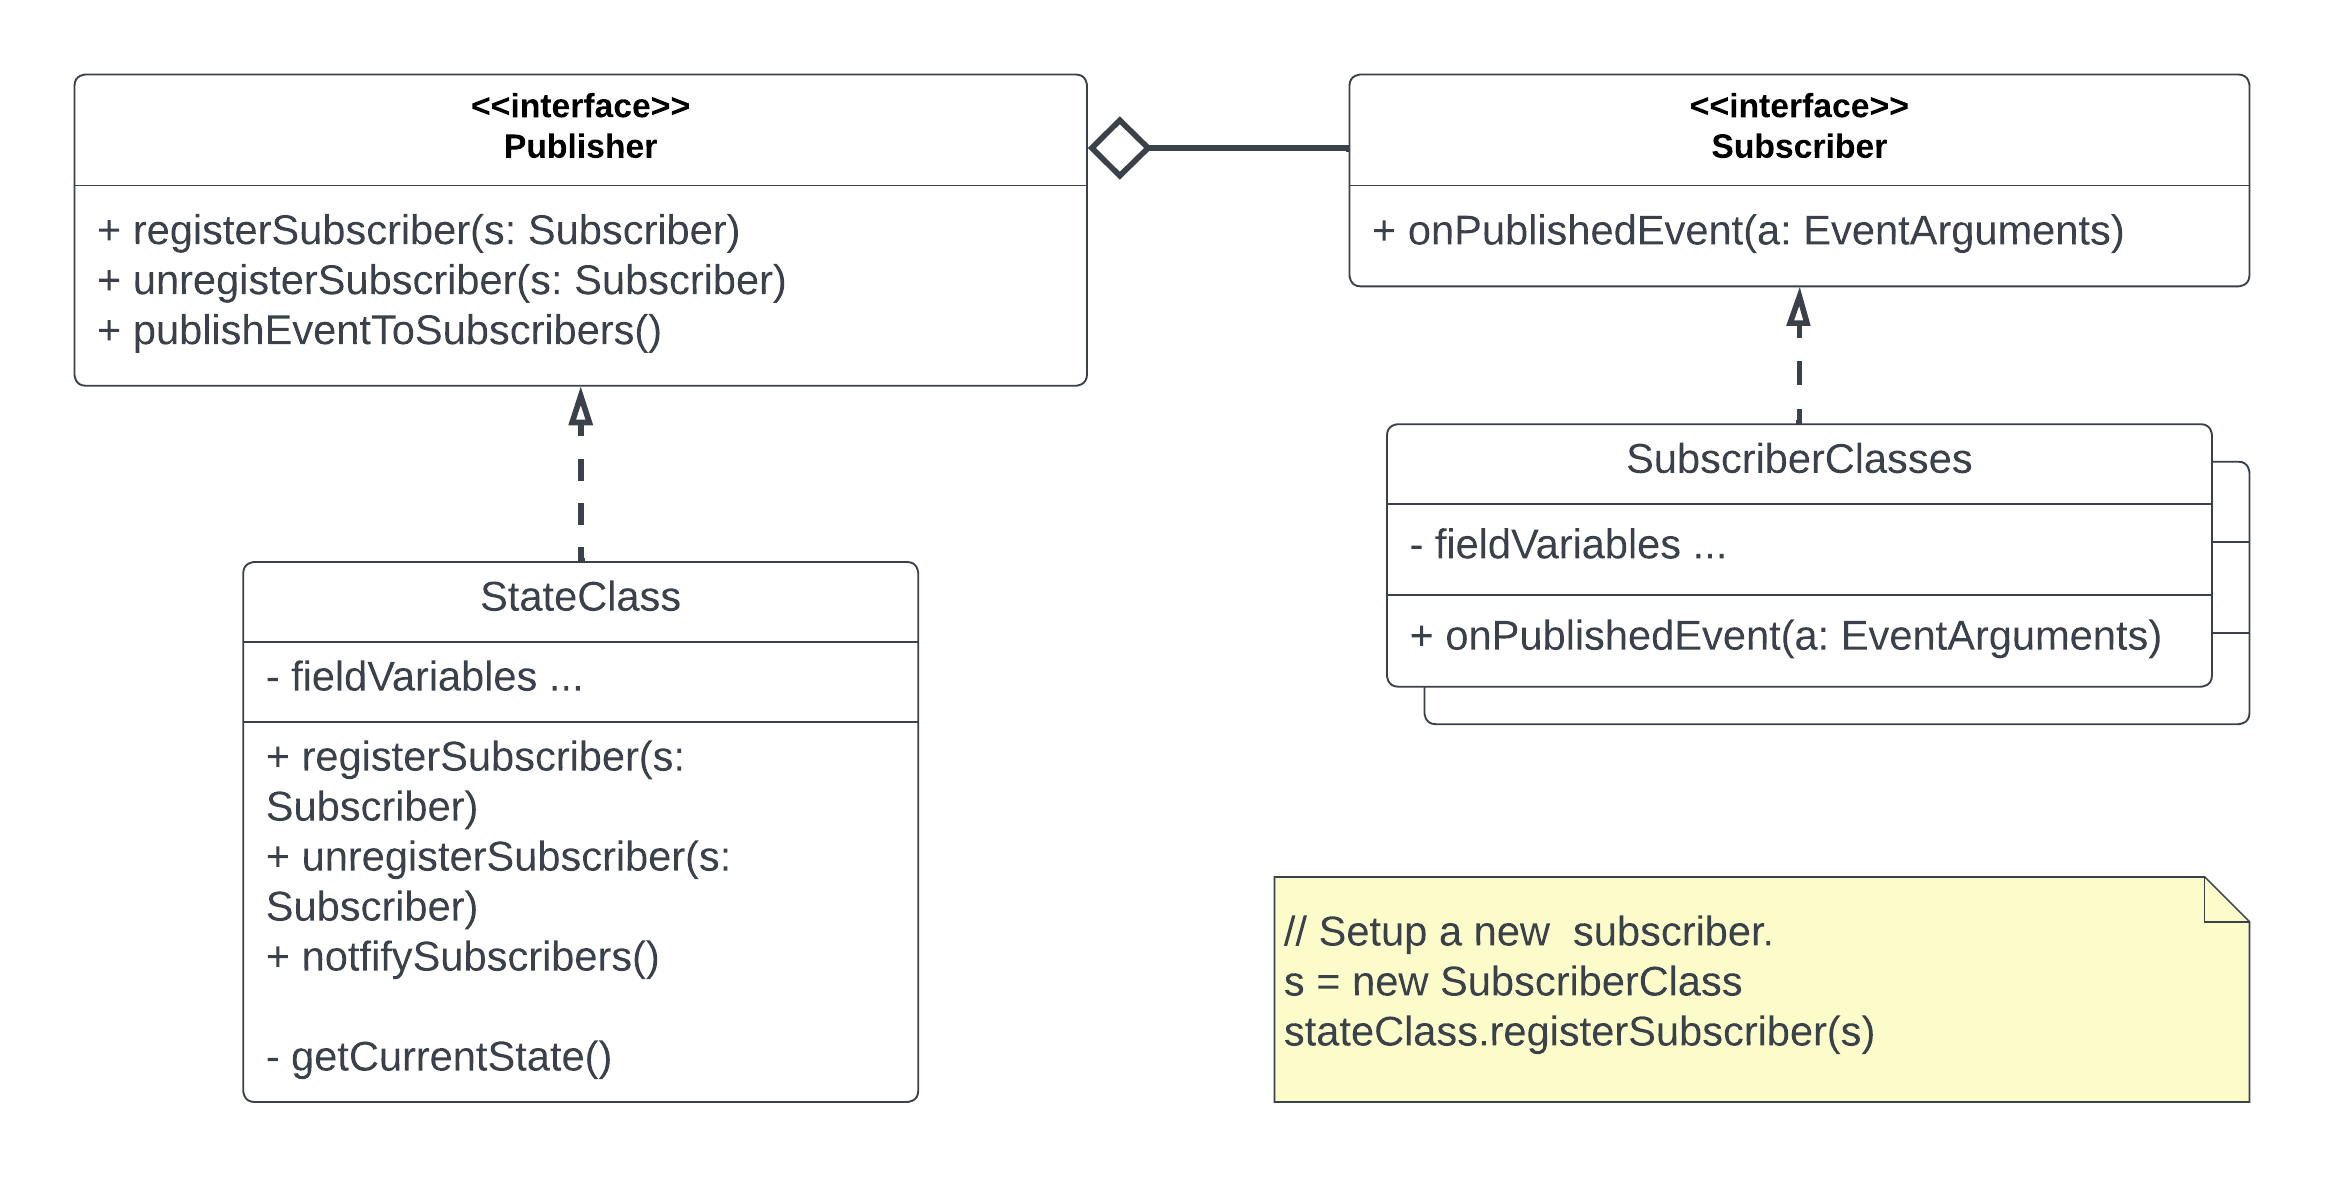
\includegraphics[scale=0.75]{Project_report/figures/theory/design_patterns/observer_uml.png}
      \caption{UML diagram of generic publisher/subscriber-relation implementation.}
      \label{fig:observer_uml}
    \end{figure}

\subsection{Overview of the Observer Pattern in Unity and C\#}
    Both the C\# programming language and the Unity API includes several features that facilitates the use of the Observer pattern. Most modern languages opt for a method-based implementation of the Observer Pattern, as compared to the class-based implementation as seen in figure \ref{fig:observer_uml}. The list that follows highlights some of the most prominent components that are used to promote the usage of this pattern:

\begin{itemize}
    \item \textbf{Delegates (C\#)}: Define a type representing a specific user-defined method signature, allowing for a method-based event system. This custom type can be realized with any method sharing the same signature as the delegate, enabling a type-safe way of passing methods as arguments. They resemble C++ function pointers but provide object-oriented capabilities by encompassing both a function and its associated object instance.
    
    \item \textbf{Event Handlers (C\#)}: Methods defined in the subscriber class that conform to a specific delegate signature, typically a delegate with two parameters: one object representing the publisher and one event data object containing event-specific information. These event handlers are responsible for processing incoming events and performing any necessary actions when the triggering event is published.
    
    \item \textbf{Events (C\#)}: A convenient feature in C\# built upon the foundation of delegates. They provide an easy way to define, subscribe, and publish events in C\#. Publishers define the event, while subscribers can subscribe or unsubscribe using the event handler. Events enforce encapsulation by allowing only the class that owns them to publish them while still enabling other classes to subscribe or unsubscribe at run-time.
    
    \item \textbf{UnityEvents (Unity)}: A built-in event class offering a flexible and powerful way to facilitate event-driven systems that can be configured in a user-friendly way through the Unity editor. Being serializable, they can easily be set up and managed through the editor using a drag-and-drop approach within the editor.
\end{itemize}

\subsection{Singleton}
    The Singleton pattern is a creational pattern that ensures only one instance of a specific class can be created at any given time, providing global access points to that instance. The pattern has garnered criticism for violating core object-oriented principles, such as The Single Responsibility Principle\footnote{The 'S' in SOLID. States that a class should only have one responsibility, promoting good separation of concern and modularity.}, promoting tight coupling, and making testing more difficult due to challenges in isolating tests, replacing instances with mocks, and managing shared global state. However, some argue for its responsible usage, applied only to classes that genuinely require a single instance and where global access is necessary. It is crucial to manage dependencies and shared states carefully to minimize the risk of creating hard-to-maintain, tightly-coupled code. Common use cases for the Singleton pattern in game development include managing access to different manager classes, such as managers for input, audio, or pooling.

    The pattern is implemented by having a private static field in the singleton class for storing the instance of the class. This instance is instantiated through a public static creation method, which uses "lazy initialization" to create a new singleton object instance through a private constructor if it is the first time the instance is being called, or returns the pre-existing instance otherwise. To ensure thread-safety in multi-threaded applications, a locking mechanism can be implemented to prevent multiple threads from creating separate instances simultaneously. This can be achieved using the "double-checked locking" pattern, where the lock is only acquired if the instance is null, reducing the performance overhead of locking in cases when the instance is already created.

    The pattern is implemented by having a private static field in the singleton class for storing the instance of the class. This instance is instantiated by having a public static creation method, that through "lazy initialization creates the new singleton object instance through a private constructor if it is the first time the instance is being called, and if not, simply returns the pre-existing instance. To ensure thread-safety in multi-threaded applications, a locking mechanism can be implemented to prevent multiple threads from creating separate instances simultaneously. This can be achieved by using the "double-checked locking" pattern, where the lock is only acquired if the instance is null, reducing the performance overhead of locking in cases when the instance is already created.

\subsection{State}
    The State pattern is a behavioral pattern that creates a modular and extensible system architecture for managing transition between different object states. The pattern does so by decoupling the logic for each possible state into a separate interface that a main class then manages by offering methods for interacting with different state objects and delegating any necessary command to the current state when told to. This main class can be described as mediator between different states, and offers the developers an user-friendly way of managing state actions and transitions.

    The pattern was first introduced by the aforementioned book "Design Patterns: Elements of Reusable Object-Oriented Software", and draws its inspiration from the concept of finite state machines (FSM) which are computational model used across a wide spectrum of domains such as control systems and artificial intelligence. A FSM consists of a finite amount of states, the initial state, and the adhering transitions between them. While both FSM and the State pattern deals with managing system behavior through various states and transition, FSM is a more general concept that focuses on the overall structure of a system, while the State pattern is a specific object-oriented concept focusing on adhering to good object-oriented principles.

    By seperating the state logic into a seperate interface, this makes it easy to accommodate for change and extensibility when modifying or adding a new state. This adheres to the Open/Closed principle\footnote{The 'O' in SOLID. Says that a class should be easy to extend without needing to modify any existing code.} as it allows developers to introduce new states without altering the existing state classes or the main class responsible for managing state transitions.

    The pattern is implemented by defining the common State interface, that should be able to handle any state specific requests and transitions. This interface is then realized by concrete states classes that provides their own unique logic and behaviour. To mediate between these states, you then implement a main class, sometimes called the Context class, that holds a reference to the current state and delegates function calls to it. This main class is also responsible for changing the current state based on transition logic defined in the concrete State classes.
    
    \begin{figure}[H]
      \centering
      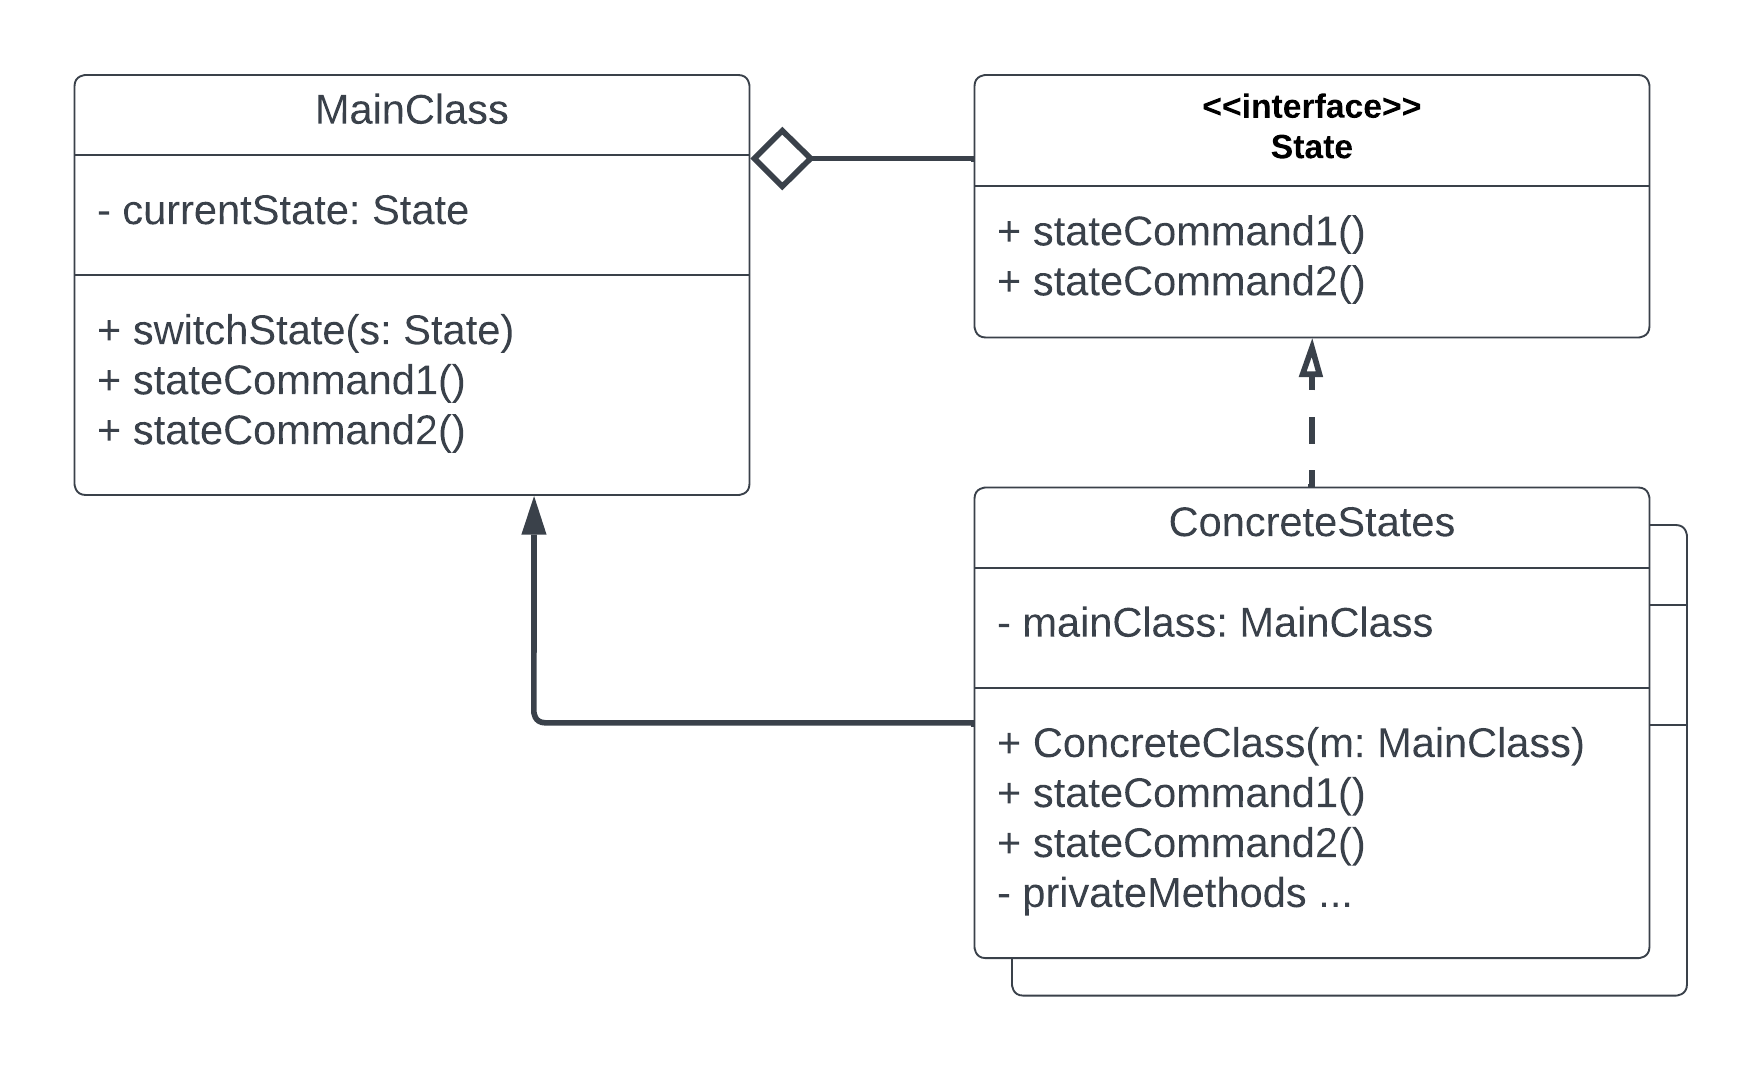
\includegraphics[scale=0.75]{Project_report/figures/theory/design_patterns/state_uml.png}
      \caption{UML diagram of generic State pattern implementation.}
      \label{fig:observer_uml}
    \end{figure}

    \vspace{50pt}
    \begin{itemize}
        \item https://www.amazon.com/-/dp/0195019199
        \item Design Patterns: Elements of Reusable Object-Oriented Software
        \item https://gameprogrammingpatterns.com/observer.html
    \end{itemize}




%% Hannes Kaulio
\section{OpenStreetMap}
    OpenStreetMap is a free database which contains geographical data. The database is maintained and updated by volunteers. Volunteers can collect data about geographical areas and add to the database for everyone to use. Data about features such as roads, railroads, buildings, trees, etc and their properties exist. 
